\documentclass[a4paper, 11pt]{article}
\usepackage{amsmath}
\usepackage{graphicx}
\usepackage{geometry}
\usepackage{listings}
\geometry{scale=0.8}

\title{	
\normalfont \normalsize
\textsc{School of Data and Computer Science, Sun Yat-sen University} \\ [25pt] %textsc small capital letters
\rule{\textwidth}{0.5pt} \\[0.4cm] % Thin top horizontal rule
\huge  The Romania Problem\\ % The assignment title
\rule{\textwidth}{2pt} \\[0.5cm] % Thick bottom horizontal rule
\author{Shixuan Lee 15336085}
\date{\normalsize\today}
}


\begin{document}
\maketitle
\newpage
\tableofcontents
\newpage
\section{codes}
\lstset{language=C++}
\lstset{breaklines=true}
\begin{lstlisting}
#include <iostream>
#include <queue>
#include <string.h>
#include <stack>
using namespace std;

int map[7][7];
string name[] = {"Arad", "Sibiu", "Remnicu_Vilcea", "Fagaras", "Craiova", "Pitesti", "Bucharest"};
const int max_n = 0x3f3f3f3f;

struct Node{
	int id;
	int cost;
	bool visit;
	int pre;
	Node(){};
	Node(bool ncity, int ncost, int nid, int npre){
		visit = ncity; cost = ncost; id = nid; pre = npre;
	}
	bool operator<(const Node &s) const{
		return cost > s.cost; 
	}
	bool operator>(const Node &s) const{
		return cost < s.cost;
	}
	bool operator==(const Node &s) const{
		return cost == s.cost;
	}
}city[7];



void initialize(){
	for(int i =0; i < 7; i++){
		for(int j = 0; j < 7; j++){
			map[i][j] = max_n;
		}
	}
	map[0][1] = map[1][0] = 140;
	map[1][2] = map[2][1] = 80;
	map[1][3] = map[3][1] = 99;
	map[2][4] = map[4][2] = 146;
	map[2][5] = map[5][2] = 97;
	map[3][6] = map[6][3] = 211;
	map[4][5] = map[5][4] = 138;
	map[5][6] = map[6][5] = 101;
	for(int k = 0; k < 7; k++){
		city[k].id = k;
		city[k].visit = 0;
	}
}

void printpath(int id){
	if(city[id].pre != -1) printpath(city[id].pre);
	cout << "-->" << name[id];
}

void searchpath(int sta, int end){
	priority_queue<Node> path;
	city[sta].cost = 0;
	city[sta].pre = -1;
	path.push(city[sta]);
	cout << "start searching path..." << endl;
	while(!path.empty()){
		int dis;
		Node temp = path.top();
		city[temp.id].visit = true;
		path.pop();
		if(temp.id == end) {
			cout << "The path is:" << endl;
			printpath(end);
			cout << endl;
			cout << "Least Cost:" << city[end].cost << endl;
			return; 
		}
		for(int i = 0; i < 7; i++){
			if(map[temp.id][i] != max_n && city[i].visit != true){
				city[i].pre = temp.id;
				city[i].cost = temp.cost + map[temp.id][i];
				path.push(city[i]);
			}
		} 	
	}
	cout << "No way to " << name[end] << endl;
}

int main(){
	initialize();
	string start, target;
	int sta , end;
	cout << "The city list:" << endl;
	for(int k = 0; k < 7; k++)
		cout << name[k] << " ";
	cout << endl; 
	cout << "Please input the start and the target:" << endl;
	cin >> start >> target;
	int i = 0;
	for(i; i < 7; i++){
		if(!start.compare(name[i])) {sta = i; break;}
	}
	if(i == 7){
		cout << "No such a city!" << endl;
		return 0;
	}
	int j = 0;
	for(j ; j < 7; j++){
		if(!target.compare(name[j])) {end = j; break;}
	}
	if(j == 7){
		cout << "No such a city!" << endl;
		return 0;
	}
	searchpath(sta, end);
	return 0;
} 





\end{lstlisting}
\section{Results}
\centering
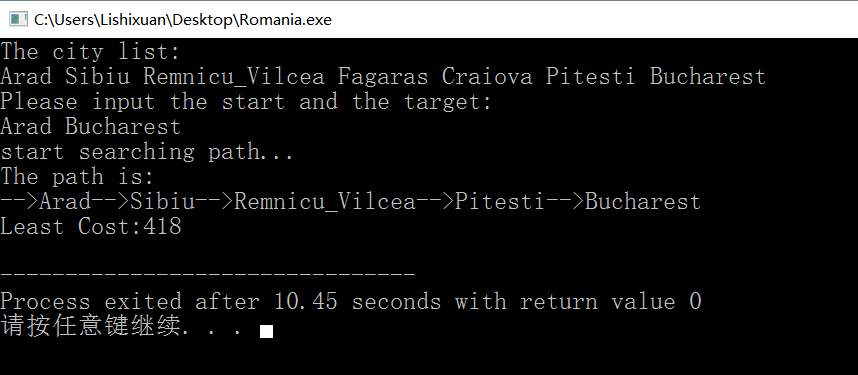
\includegraphics[width=15cm]{Romania.png}
%\tableofcontents
%\newpage

\end{document} 